% !TEX root = ../main.tex
\chapter{车道汇合场景的单车最优控制}
\label{cha:solve}

在上一章中已经给出了模型的目标函数,并且提到需要对每辆车求解一个控制量输入$u_i(t)$,使得$J(\bm{u})$达到最小。注意到$u_t(t)$实际上是关于时间$t$的函数,$J(\bm{u})$实际上是函数的函数,数学上称为泛函。求泛函的极值需要用到变分法的相关知识。本章先对泛函与变分法进行简要说明,之后运用该方法求解不同情况下泛函的极值,得到决策控制方法。

\section{泛函与变分法}
泛函的概念最早在变分法中出现,并广泛应用于最优控制的相关问题中。

\subsection{泛函与泛函的变分}
抽象空间理论将泛函定义为向量空间上的实值函数,而在最优控制中往往限定为函数集上的实值函数。定义如下,
\begin{definition}[泛函]
函数集$\mathcal{U}(x)$,到实数集$\mathbb{R}$的映射$J: \mathcal{U}\rightarrow \mathbb{R}$称为函数集$\mathcal{U}$上的{\heiti 泛函},即,
\begin{equation}
J=J[u(x)], \ u(x)\in \mathcal{U}(x).
\end{equation}
\end{definition}
泛函的变分与函数的微分类似。首先需要定义函数的变分,定义如下:
\begin{definition}[函数的变分]
设$u(x), u_0(x) \in \mathcal{U}(x)$,{\heiti 函数的变分}定义为
\begin{equation}
\delta u(x)=u(x) - u_0(x).
\end{equation}
\end{definition}
由以上定义知,函数的变分仍是$x$的函数。另外根据泛函定义,函数集$\mathcal{U}(x)$应是向量空间,对加法和数乘封闭,因此$\delta u(x)\in \mathcal{U}(x)$。
之后定义泛函的连续性如下,
\begin{definition}[泛函的连续性]
$\forall \varepsilon > 0$,$\exists \delta > 0$,对于$\forall u(x), d(u,u_0)<\delta$有
\begin{equation}
\Delta J[u(x)]=J[u(x)+\delta u(x)]-J[u(x)] < \delta,
\end{equation}
其中$d(u,u_0)$为函数空间$\mathcal{U}$上定义的某种范数,则称泛函$J[u(x)]$在范数$d$下,在$u_0(x)$连续。
\end{definition}
泛函的变分定义如下,
\begin{definition}[泛函的变分]
泛函的增量若能表示为
\begin{equation}
\Delta J[u(x)]=L[u(x),\delta u(x)] + \gamma[u(x), \delta u(x)],
\end{equation}
其中$L[u(x),\delta u(x)]$是$\delta u(x)$的线性连续泛函,$\gamma[u(x), \delta u(x)]$是$\delta u(x)$的高阶无穷小,则称$L[u(x),\delta u(x)]$为泛函$J[u(x)]$的变分,记为
\begin{equation}
\delta J = L[u(x),\delta u(x)].
\end{equation}
\end{definition}
关于线性连续泛函的概念,以及泛函变分更严谨的定义,参见泛函分析的教材\cite{PETERD2007Functional}。

\subsection{变分法}
求泛函极值的方法称为变分法。泛函极值的定义与函数极值类似。下面不加证明地给出如下定理:
\begin{theorem}
若泛函$J[u(x)]$在$u_0(x)$有极值,则
\begin{equation}
\delta J[u_0(x)]=0.
\end{equation}
\end{theorem}
注意,上述定理只是泛函取极值的必要条件。至于是否存在极值,是极大还是极小值,需要根据实际问题的性质确定。

变分学中有如下三类基本问题。三者区别在于泛函形式不同,而目标都是求泛函极小值。

\textbf{拉格朗日(Lagrange)问题} \ \ 泛函形式为
\begin{equation}
J = \int_{t_0}^{t_\mathrm{f}}F(t,x,\dot{x})\mathrm{d}t,
\end{equation}
其中$t_0$为初始时间,$t_f$为终端时间。

\textbf{梅耶(Mayer)问题} \ \ 泛函形式为
\begin{equation}
J=\theta[x_\mathrm{f},t_\mathrm{f}].
\end{equation}
该泛函是终端时间$t_\mathrm{f}$和终端函数$x_\mathrm{f}=x(t_mathrm{f})$的函数。

\textbf{波尔查(Bolza)问题} \ \ 泛函形式为
\begin{equation}
J=\theta[x_\mathrm{f},t_\mathrm{f}]+\int_{t_0}^{t_\mathrm{f}}F(t,x,\dot{x})\mathrm{d}t.
\end{equation}
可见,前两者是后者的特殊形式。

\subsection{最优控制的必要条件}
最优控制问题常写作如下形式的波尔查问题
\begin{equation}
J(\bm{u})=\theta[t_\mathrm{f},\bm{x}_\mathrm{f}]+\int_{t_0}^{t_\mathrm{f}}L[\bm{x}(t),\bm{u}(t),t]\mathrm{d}t,
\end{equation}
其状态方程和初始状态为
\begin{equation}
\dot{\bm{x}}=\bm{f}[\bm{x}(t),\bm{u}(t),t], \quad \bm{x}(t_0)=\bm{x}_0.
\end{equation}
定义{\heiti 哈密顿函数}为
\begin{equation}
H(\bm{x},\bm{u},\bm{\lambda},t)=L(\bm{x},\bm{u},t)+\bm{\lambda}^\mathrm{T}\bm{f}(\bm{x},\bm{u},t),
\end{equation}

下面针对上述波尔查问题的形式,给出几种情况下的最优控制必要条件。若最优控制的损失函数退化为拉格朗日或梅耶问题的形式,其必要条件也可以相应得出。
\\
\begin{enumerate}[wide=\parindent]
\item {\heiti 终端自由,$t_\mathrm{f}$给定的情形}

最优控制的必要条件为
\begin{gather}
\frac{\partial H}{\partial\bm{u}}=0,\label{eq:nc:control}\\
\dot{\bm{\lambda}}=-\frac{\partial H}{\partial\bm{x}},\label{eq:nc:company}\\
\bm{\lambda}(t_\mathrm{f})=\left. \left[\frac{\partial \theta}{\partial \bm{x}}+\frac{\partial \bm{g}^\mathrm{T}}{\partial \bm{x}}\bm{\mu}\right]\right|_{t_\mathrm{f}},\label{eq:nc:final}\\
\dot{\bm{x}}=\bm{f}(\bm{x},\bm{u},t),\\
\bm{x}(t_0)=\bm{x}_0.\label{eq:nc:last}
\end{gather}
其中式\eqref{eq:nc:control}也被称作{\heiti 控制方程},式\eqref{eq:nc:company}也被称作{\heiti 伴随方程}。若退化为拉格朗日问题,则$\theta[t_\mathrm{f},\bm{x}_\mathrm{f}]\equiv 0$,式\eqref{eq:nc:company}变为
\begin{equation}
\bm{\lambda}(t_\mathrm{f})=0.
\end{equation}

\item {\heiti 终端受限,$t_\mathrm{f}$给定的情形}

设终端约束条件为
\begin{equation}
\bm{g}(\bm{x}_\mathrm{f},t_\mathrm{f})=0,
\end{equation}
最优控制的必要条件为
\begin{gather}
\frac{\partial H}{\partial\bm{u}}=0,\label{eq:cc:control}\\
\dot{\bm{\lambda}}=-\frac{\partial H}{\partial\bm{x}},\label{eq:cc:company}\\
\bm{\lambda}(t_\mathrm{f})=\left. [\frac{\partial \theta}{\partial \bm{x}}+\frac{\partial \bm{g}^\mathrm{T}}{\partial \bm{x}}\bm{\mu}]\right|_{t_\mathrm{f}},\label{eq:cc:final}\\
\dot{\bm{x}}=\bm{f}(\bm{x},\bm{u},t),\\
\bm{x}(t_0)=\bm{x}_0.\label{eq:cc:last}
\end{gather}
其中$\bm{\mu}$为一个待定乘子。对比式\eqref{eq:cc:final}与式\eqref{eq:nc:final}可知,终端受限情况下,终端条件会发生变化。

\item {\heiti 终端受限,$t_\mathrm{f}$自由的情形}

最优控制的必要条件为
\begin{gather}
\frac{\partial H}{\partial\bm{u}}=0,\label{eq:cn:control}\\
\dot{\bm{\lambda}}=-\frac{\partial H}{\partial\bm{x}},\label{eq:cn:company}\\
\bm{\lambda}(t_\mathrm{f})=\left. \left[\frac{\partial \theta}{\partial \bm{x}}+\frac{\partial \bm{g}^\mathrm{T}}{\partial \bm{x}}\bm{\mu}\right]\right|_{t_\mathrm{f}},\label{eq:cn:final}\\
\left. \left[H+\frac{\partial\theta}{\partial t}+\bm{\mu}^\mathrm{T}\frac{\partial\bm{g}}{\partial t}\right]\right|_{t_\mathrm{f}}=0,\label{eq:cn:final2}\\
\dot{\bm{x}}=\bm{f}(\bm{x},\bm{u},t),\\
\bm{x}(t_0)=\bm{x}_0.\label{eq:cn:last}
\end{gather}
与之前的情形相比,该情形多了一个终端条件以确定$t_\mathrm{f}$。
\end{enumerate}

\section{最优控制问题求解}
\label{sec:solve}
运用上述最优控制的必要条件,可求解本课题的车道汇合群决策模型,获得最优控制策略。下面三小节分别考虑三种情形,其中\ref{ssec:noc}节首先研究控制量和状态量无约束,且终端时间固定的简单情形;\ref{ssec:freetf}节研究控制量和状态量无约束,终端时间自由的情形;\ref{ssec:c}研究控制量和状态量存在约束的情形。

\subsection{控制系统无约束}
\label{ssec:noc}
本节中的无约束是指对每辆CAV均不限制最大加速度和速度。另外,终端时间事先给定。式\eqref{eq:one_item_obj}在这种情形下,设$t_i^{0}=0$并省略所有下标$i$,最优控制问题的形式为
\begin{gather}
\min_{u} J(u)=\int_{0}^{t^\mathrm{m}}L(p,v,u,t)\mathrm{d}t=\int_{0}^{t^\mathrm{m}}\frac12 u^2\mathrm{d}t,\label{eq:noc:first}\\
p(0)=0, v(0)=v_0,\label{eq:noc:start}\\
p(t^\mathrm{m})=L, v(t_\mathrm{m})=v_\mathrm{d},\label{eq:noc:end}\\
\dot{p}=v, \dot{v}=u, \label{eq:noc:last}
\end{gather}
其中式\eqref{eq:noc:first}为目标函数,式\eqref{eq:noc:start}为初始状态,式\eqref{eq:noc:end}为终端约束,式\eqref{eq:cc:last}为系统状态方程。该问题是终端受限,$t_\mathrm{f}$给定的最优控制问题,必要条件为式\eqref{eq:cc:control}--- 式\eqref{eq:cc:last}。该问题的哈密尔顿函数为,
\begin{equation}
H(p,v,u,t)=\frac12 u^2+\lambda^\mathrm{p}v + \lambda^\mathrm{v}u.
\end{equation}
由伴随方程得
\begin{align}
\dot{\lambda}^\mathrm{p}&=-\frac{\partial H}{\partial p}=0, \label{eq:dlp}\\
\dot{\lambda}^\mathrm{v}&=-\frac{\partial H}{\partial v}=-\lambda^\mathrm{p}. \label{eq:dlv}
\end{align}
由控制方程可得
\begin{equation}
\frac{\partial H}{\partial u}=u+\lambda^\mathrm{v}=0.
\label{eq:uwrtlv}
\end{equation}

式\eqref{eq:dlp}说明$\lambda^\mathrm{p}$为常数,设$\lambda^\mathrm{p}=a$,则可设$\lambda^\mathrm{v}=-(at+b)$,再由式\eqref{eq:uwrtlv}可得
\begin{equation}
u^*(t)=at+b.
\label{eq:ut}
\end{equation}
即在该情形下,最优的控制策略是加速度为时间的线性函数。注意在终端受限,$t_\mathrm{f}$自由情形的必要条件中还有关于$\bm{\lambda}$末状态的方程,但该方程额外引入了待定参数$\bm{\mu}$,实际上对求解最优控制不起作用,因此无需列出。
在该控制策略下,速度和位移与时间的关系可分别表达为时间的二次、三次函数
\begin{gather}
v^*(t)=\frac12at^2+bt+c,\\
p^*(t)=\frac16at^3+\frac12bt^2+ct+d.
\end{gather}
以上$a,b,c,d$均为待定常数,可以根据初始条件式\eqref{eq:noc:start}和终端条件式\eqref{eq:noc:end}得出。可列写如下方程
\begin{equation}
\begin{bmatrix}
\frac16t^3 & \frac12t^2 & t & 1 \\
\frac12t^2 & t & 1 & 0 \\
\frac16(t^\mathrm{m})^3 & \frac12(t^\mathrm{m})^2 & t^\mathrm{m} & 1 \\
\frac12(t^\mathrm{m})^2 & t^\mathrm{m} & 1 & 0
\end{bmatrix}\cdot
\begin{bmatrix}
a\\b\\c\\d
\end{bmatrix}
 = \begin{bmatrix}
p(t)\\v(t)\\p(t^\mathrm{m})\\v(t^\mathrm{m})
\end{bmatrix}.
\label{eq:noc:array}
\end{equation}
令$t$为进入控制区的时刻,则可以由初末状态,根据以上方程解出参数。注意,以上方程对每辆CAV都可以单独列写,即每辆车单独计算自己的控制策略。

\subsection{终端时间自由}
\label{ssec:freetf}
在第\ref{ssec:time_series}节曾提到,对于头一辆车,终端时间是待定的,而后面的车辆可以在预先确定通过顺序的情况下,由前一辆车的通过时间按照式\eqref{eq:t_case1},式\eqref{eq:t_case2}(或式\eqref{eq:t_case2r})确定。头一辆车的优化问题是一个终端受限,$t_\mathrm{f}$自由的最优控制问题,必要条件为式\eqref{eq:cn:control} $\sim$ 式\eqref{eq:cn:last}。问题的表述如式\eqref{eq:noc:first} $\sim$ 式\eqref{eq:noc:last}。这里将末态约束写为向量函数式
\begin{equation}
\bm{g}(p(t^\mathrm{m}),v(t^\mathrm{m}),t^\mathrm{m})=
\begin{bmatrix}
p(t^\mathrm{m})-L\\
v(t^\mathrm{m})-v_\mathrm{d}
\end{bmatrix}.
\end{equation}
由伴随方程和控制方程仍可解出$u(t)$为线性形式,如式\eqref{eq:ut}。下面需要终端方程来确定$t^\mathrm{m}$。

由终端条件式\eqref{eq:cn:final}和式\eqref{eq:cn:final2},
\begin{align}
\lambda^\mathrm{p}(t^\mathrm{m})=\frac{\partial \bm{g}^\mathrm{T}}{\partial p}\bm{\mu}=\mu^\mathrm{p},\label{eq:freetf:f1}\\
\lambda^\mathrm{v}(t^\mathrm{m})=\frac{\partial \bm{g}^\mathrm{T}}{\partial v}\bm{\mu}=\mu^\mathrm{v},\label{eq:freetf:f2}\\
\left. H+\mu^\mathrm{p}v+\mu^\mathrm{v}u\right|_{t^\mathrm{m}}=0.\label{eq:freetf:f3}
\end{align}
将式\eqref{eq:freetf:f1},式\eqref{eq:freetf:f2}及$u=-\lambda^\mathrm{v}$代入式\eqref{eq:freetf:f3},整理得
\begin{equation}
-\frac32(\lambda^\mathrm{v}(t^\mathrm{m}))^2+2\lambda^\mathrm{p}(t^\mathrm{m})v^\mathrm{m}=0,
\label{eq:freetf:tf}
\end{equation}
其中$v^\mathrm{m}$为末态速度,在当前情形下,$v^\mathrm{m}=v_\mathrm{d}$已经给定。由式\eqref{eq:freetf:tf},再结合方程组式\eqref{eq:noc:array},即可解出$a,b,c,d,t^\mathrm{m}$。

上述方程组实际上已经是四次方程组,解的情况十分复杂。仿真中发现,大多数数值计算软件包(如{\ttfamily Python}的{\ttfamily sympy}包,{\ttfamily Mathematica}等)在实数解存在的情况下也不能保证找到可行的解。因此,实际求解过程中用$t^\mathrm{m}$表示目标函数,并直接求极值来求解$t^\mathrm{m}$。由式\eqref{eq:noc:array}可解得
\begin{equation}
\begin{aligned}
a &= \frac{12t^\mathrm{m} (p_0 - L + t^\mathrm{m}v_0) - 6(t^\mathrm{m})^2(v_0 - v_\mathrm{m})}{(t^\mathrm{m})^4},\\
b &= -\frac{6(p_0 - L) + 4t^\mathrm{m}v_0 + 2t^\mathrm{m}v_\mathrm{m}}{(t^\mathrm{m})^2},
\end{aligned}
\label{eq:abwrttm}
\end{equation}
式中$p_0=p(t^0)$,$v_0=v(t^0)$,$L=p(t^\mathrm{m})$,$v_\mathrm{m}=v(t^\mathrm{m})$。将式\eqref{eq:ut}代入目标函数式\eqref{eq:one_item_obj},并求取原函数,可得
\begin{equation}
J=\left.\frac12(\frac13a^2t^3+abt^2+b^2t)\right|^{t^\mathrm{m}}_{t^0}.
\label{eq:tmopt}
\end{equation}
将式\eqref{eq:abwrttm}代入上式,即可将目标函数$J$表示为$t^\mathrm{m}$的函数$J(t^\mathrm{m})$,由此可以通过数值方法确定$J(t^\mathrm{m})$的极值以及取极值时的$t^\mathrm{m}$。

\begin{figure}
\centering
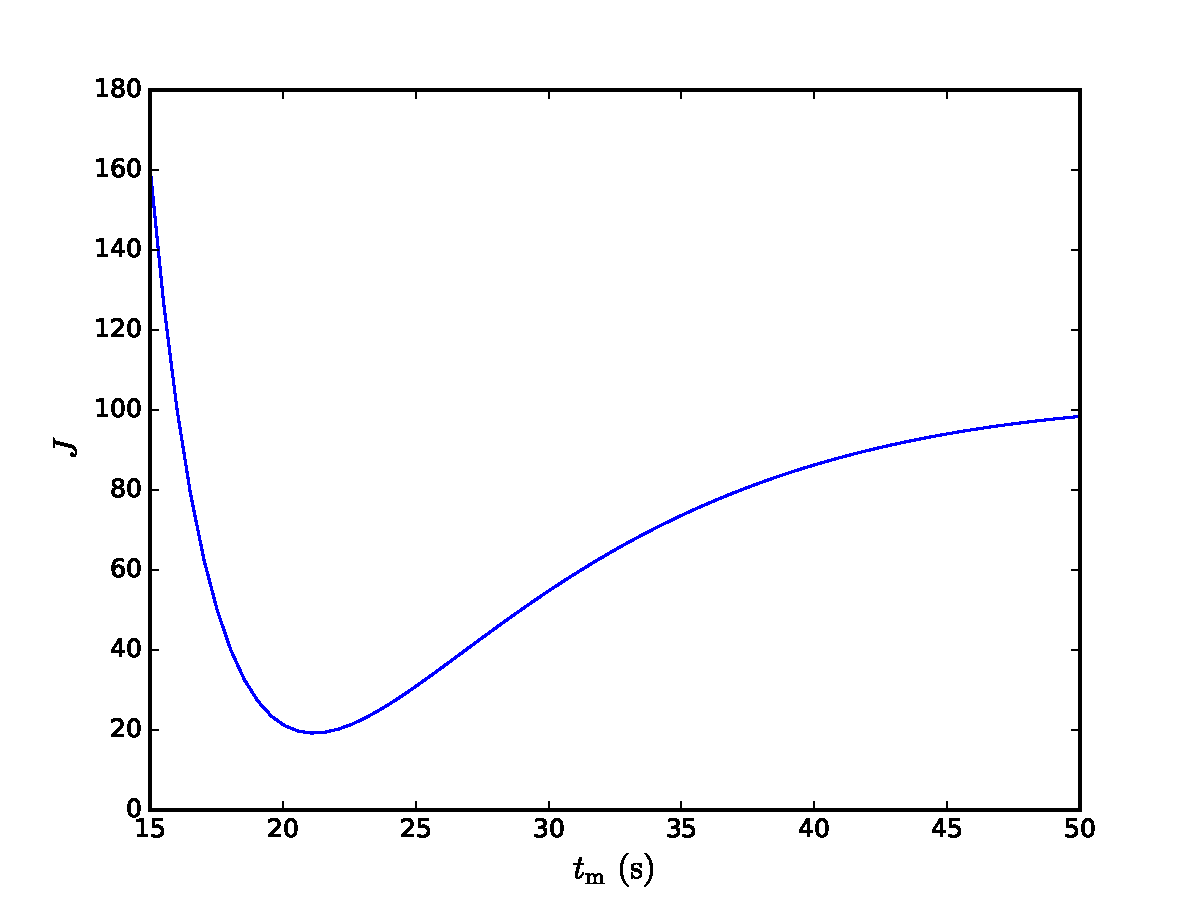
\includegraphics[width=10cm]{figures/tm.pdf}
\caption{$J\sim t_\mathrm{m}$关系曲线}
\label{fig:tm}
\end{figure}

图\ref{fig:tm}做出了$p_0=0$,$v_0=\SI{13.4}{m\per s}$,$L=\SI{400}{m}$,$v_\mathrm{m}=\SI{25.0}{m\per s}$条件下的$J\sim t_\mathrm{m}$关系曲线。经实验发现,在正常范围内,$J\sim t_\mathrm{m}$都是形如图\ref{fig:tm}的图线,很容易找到极小值。

\subsection{控制系统有约束}
\label{ssec:c}
考虑速度、加速度的约束,某辆车的哈密尔顿函数为
\begin{multline}
H(p,v,u,t)=\frac12u^2+\lambda^\mathrm{p}v + \lambda^\mathrm{v}u+\\
\mu^\mathrm{a}(u-u_{\max})+\mu^\mathrm{b}(u_{\min}-u)+\mu^\mathrm{c}(v-v_{\max})+\mu^\mathrm{d}(v_{\min}-v),
\end{multline}
其中,$\mu^\mathrm{a},\mu^\mathrm{b},\mu^\mathrm{c}\mu^\mathrm{d}$为拉格朗日乘子,
\begin{align}
\mu^\mathrm{a}=\begin{dcases}
>0, & u(t)-u_{\max}=0,\\
=0, & u(t)-u_{\max}<0,
\end{dcases}\\
\mu^\mathrm{b}=\begin{dcases}
>0, & u_{\min}-u(t)=0,\\
=0, & u_{\min}-u(t)<0,
\end{dcases}\\
\mu^\mathrm{c}=\begin{dcases}
>0, & v(t)-v_{\max}=0,\\
=0, & v(t)-v_{\max}<0,
\end{dcases}\\
\mu^\mathrm{d}=\begin{dcases}
>0, & v_{\min}-v(t)=0,\\
=0, & v_{\min}-v(t)<0.
\end{dcases}
\end{align}
由伴随方程,
\begin{gather}
\lambda^\mathrm{p}=-\frac{\partial H}{\partial p} = 0,\\
\lambda^\mathrm{v}=-\frac{\partial H}{\partial v} =
\begin{dcases}
-\lambda^\mathrm{p}, & v(t)-v_{\max}<0 \quad \text{and}\\ & v_{\min}-v(t)<0,\\
-\lambda^\mathrm{p}-\mu^\mathrm{c}, & v(t)-v_{\max}=0,\\
-\lambda^\mathrm{p}+\mu^\mathrm{d}, & v_{\min}-v(t)=0.
\end{dcases}
\end{gather}
由控制方程,
\begin{equation}
\frac{\partial H}{\partial u}=u+\lambda^\mathrm{v}+\mu^\mathrm{a}-\mu^\mathrm{b}=0.
\end{equation}
下面根据是否触发约束条件分情况讨论。
\begin{enumerate}[label=(\arabic*),wide=\parindent]
% \begin{enumerate}
\item 未触发约束条件。这时哈密尔顿函数退化为\ref{ssec:noc}节所述的情形,因此最优控制为式\eqref{eq:ut}。
\item 触发约束条件,$u(t)=u_{\max}$且$v_{\min}<v(t)<v_{\max}$。假设在$t=t_1$时,该条件成立,则对于$\forall t>t_1$,
\begin{gather}
u^*(t)=u_{\max},\\
v^*(t)=u_{\max}t+f,\\
p^*(t)=\frac12u_{\max}t^2+ft+e.
\end{gather}
即车辆应按照最大加速度继续运行。其中参数$f$和$e$可由车辆在$t=t_1$时刻的位置和速度解出。
\item 触发约束条件,$u(t)=u_{\max}$且$v(t)=v_{\max}$,假设在$t=t_2>=t_1$时,$v(t)=v_{\max}$成立,则对于$\forall t>t_2$,
\begin{gather}
v^*(t)=v_{\max},\\
p^*(t)=v_{\max}t+q,\\
u^*(t)=\dot{v}^*(t)=0.
\end{gather}
车辆按照最大速度运行。其中参数$q$可由$t=t_2$时刻的位置解出。进一步地,如果在$t=t_3$时刻,车辆退出了该情况,即$v_{\min}<v(t)<v_{\max}$,则此时加速度应当重新回到线性形式,即
\begin{gather}
u^*(t)=gt+h,\label{eq:noc:lo1}\\
v^*(t)=\frac12gt^2+ht+r,\\
p^*(t)=\frac16gt^3+\frac12ht^2+rt+s.\label{eq:noc:lo3}
\end{gather}
其中参数$g$,$h$,$r$和$s$可仿照式\eqref{eq:noc:array}由该段初末状态解出。

\item 触发约束条件,$u(t)=u_{\min}$且$v_{\min}<v(t)<v_{\max}$。假设在$t=t_1$时,该条件成立,则对于$\forall t>t_1$,
\begin{gather}
u^*(t)=u_{\max},\\
v^*(t)=u_{\max}t+f,\\
p^*(t)=\frac12u_{\max}t^2+ft+e.
\end{gather}
即车辆应按照最大加速度减速运行。其中参数$f$和$e$可由车辆在$t=t_1$时刻的位置和速度解出。
\item 触发约束条件,$u(t)=u_{\min}$且$v(t)=v_{\min}$,假设在$t=t_2>=t_1$时,$v(t)=v_{\min}$成立,则对于$\forall t>t_2$,
\begin{gather}
v^*(t)=v_{\min},\\
p^*(t)=v_{\min}t+q,\\
u^*(t)=\dot{v}^*(t)=0.
\end{gather}
车辆按照最小速度运行。其中参数$q$可由$t=t_2$时刻的位置解出。进一步地,如果在$t=t_3$时刻,车辆退出了该情况,即$v_{\min}<v(t)<v_{\max}$,则此时加速度应当重新回到线性形式,最优控制由式\eqref{eq:noc:lo1}--- 式\eqref{eq:noc:lo3}给出。
\item 触发约束条件,$v(t)=v_{\max}$且$u_{\min}<u(t)<u_{\max}$,假设在$t=t_2>=t_1$时,该条件成立,则对于$\forall t>t_2$,
\begin{gather}
v^*(t)=v_{\max},\\
p^*(t)=v_{\max}t+q,\\
u^*(t)=\dot{v}^*(t)=0.
\end{gather}
车辆按照最大速度运行。其中参数$q$可由$t=t_2$时刻的位置解出。进一步地,如果在$t=t_3$时刻,车辆退出了该情况,即$v_{\min}<v(t)<v_{\max}$,则此时加速度应当重新回到线性形式,最优控制由式\eqref{eq:noc:lo1}--- 式\eqref{eq:noc:lo3}给出。
\item 触发约束条件,$v(t)=v_{\min}$且$u_{\min}<u(t)<u_{\max}$,假设在$t=t_2>=t_1$时,该条件成立,则对于$\forall t>t_2$,
\begin{gather}
v^*(t)=v_{\min},\\
p^*(t)=v_{\min}t+q,\\
u^*(t)=\dot{v}^*(t)=0.
\end{gather}
车辆按照最小速度运行。其中参数$q$可由$t=t_2$时刻的位置解出。进一步地,如果在$t=t_3$时刻,车辆退出了该情况,即$v_{\min}<v(t)<v_{\max}$,则此时加速度应当重新回到线性形式,最优控制由式\eqref{eq:noc:lo1}--- 式\eqref{eq:noc:lo3}给出。
\end{enumerate}
\begin{remark}
对于以上讨论的触发约束的情况,按照约束值运行可以保证满足最优控制的必要条件。如果在某时刻退出了约束状态,只要后半段控制量为线性形式,仍然可以保证满足必要条件。由此可见,上述最优控制理论只给出了控制量的形式,至于某个控制序列是否为最优控制,还需要其他方式进行判断。在\ref{sec:cc}节将要给出具体的解的形式,并使用数值解法求解优化问题,给出最优控制。
% \begin{enumerate}
% \item $t_i^c < t_{k} + \frac{\delta}{v_k^m}$, 按式(14),$t_i^{m*}=t_{k} + \frac{\delta}{v_k^m}$;
% \item 按照式(33)解最优控制发现超速,这时按下界走又会撞前车。此时应该怎样控制?
% \end{enumerate}
\end{remark}